\chapter{Analysephase}

\section{Expected Goals}
\label{goals}
Dieser Abschnitt soll dem Leser den aktuellen Forschungsstand der \textit{Expected Goals} vermitteln, deren Bedeutsamkeit für den Fußballsport dabei explizit aufzeigen, sowie den Einfluss von Data-Mining-Methoden hinsichtlich der Wissensgewinnung darstellen.

\begin{quote}
\textit{\glqq Expected Goals - Das angesagteste Statistikmodell im Profifußball\grqq}
\end{quote}

So betitelt Nils Nordmann seinen Online-Artikel im Interview mit Dustin Böttger, Geschäftsführer von \gls{gsn}, einem der gefragtesten Datenanalysten aus Deutschland, der mit mehreren Bundesligavereinen in Kooperation steht.\seFootcite{}{}{NilsNordmann.2016} Statistische Analysen sind im Bereich des Fußballs keine Neuheit mehr, jedoch liegt der Ursprung der sportlichen Datenanalyse in einer anderen Sportart. Der amerikanische Historiker und Statistiker Bill James veröffentlichte 1977 erste Analysen zwischen geschlagenen und gefangenen Bällen im Baseball, um eine objektive Bewertung der Gesamtleistung eines Spielers aufstellen zu können. Schumaker, Solieman und Chen bezeichnen diese Entwicklung als eine Art \glqq Revolution\grqq-- einen Wandel von traditionellen Statistiken hin zum Wissensmanagement.\seFootcite{Vgl.}{S.36}{Schumaker.2010} Diese löste eine Welle der Erstellung neuer Maßzahlen aus, wovon einige im Jahr 2002 von der amerikanischen Baseball Profimannschaft \textit{Oakland A’s Billy Bean} als Grundlage zur Zusammenstellung eines neuen Teams dienten. Die \textit{Boston Red Sox} ließen sich von dieser Idee inspirieren und  gewannen anschließend sogar 2004 und 2007 die Meisterschaft.\seFootcite{Vgl.}{S.36}{Schumaker.2010} Auch aus anderen Sportarten gibt es vergleichbare Beispiele, wie die digitale Revolution im Basketball im Jahr 1980 durch den Statistiker Dean Oliver, der neue Messwerte zur Beurteilung von Spielern veröffentlichte.\footnote{Dean Oliver beriet 2005 die \textit{Seatlle Supersonics} und verhalf zur amerikanischen Meisterschaft}

Waren im Fußball in der Vergangenheit noch rein quantitative \glspl{kpi} wie der Ballbesitz, die Passquote oder die Anzahl der Torschüsse von Bedeutung, wird das Spiel heutzutage bis in das kleinste Detail (z.B. die Anzahl der vertikal \glqq überspielten\grqq~Gegenspieler durch einen Pass) analysiert. Durch den Fortschritt der Videotechnik können alle Aktionen eines Spieles aufgezeichnet werden, wodurch sich neue stichhaltige Bewertungsmethoden herauskristallisiert haben. Sumpter, Anderson und weitere Fachexperten untersuchen mit Hilfe von Mathematik und Statistik das Spiel und stellen in ihren Ausführungen einige Thesen und Modelle auf.\seFootcite{Vgl.}{}{Sumpter.2016}\seFootcite{Vgl.}{}{Anderson.2014}\seFootcite{Vgl.}{}{Heuer.2010} Eines der momentan angesagten Modelle ist das der \glqq \textbf{Expected Goals}\grqq (\textit{dt. die zu erwartenden Tore}), welches die Qualität von Torschüssen vielseitig, objektiv und plausibel misst.\seFootcite{}{}{NilsNordmann.2016} Dazu wird jedem Schuss, unter der Berücksichtigung von Parametern (wie beispielsweise der Position oder des Körperteils mit dem geschossen wurde), eine bestimmte Erfolgswahrscheinlichkeit zugewiesen. Die Bestimmung der Wahrscheinlichkeit, die Auswahl der einbezogenen Schüsse wie auch Parameter und teilweise das gesamte Modell wird öffentlich von den Analytikern (meist aus Unternehmen der Sportanalyse/-beratung) nur kurz ausgeführt oder gar komplett geheimgehalten. Einblicke in ihre Modellierungen bieten unter anderem Opta Sports\seFootcite{Vgl.}{}{PhilippObloch.2015}, der TV-Sender Sky Sports,\seFootcite{Vgl.}{}{PhilippErtl.2016} oder Experten, wie Michael Caley, in ihren Internetpublikationen.\seFootcite{Vgl.}{}{MichaelCaley.2017} Ein \textit{Expected-Goal-Modell} offeriert eine statistisch belegte und damit objektive Bewertung von Schüssen und bildet einen neuen \gls{kpi} bezüglich der Qualität einer Torchance. Anhand dieser Grundlage ist es möglich, weitere Bewertungsmethoden für Spieler und Mannschaften zu ermitteln, die vor allem im Scouting-Bereich ihre Anwendung finden. Durch die qualitative Bewertung der Schüsse eines Stürmers mittels des Expected-Goal-Modells, kann eine objektive Aussage über dessen Erfolgsquote getroffen werden (beispielsweise ob diese über den erwarteten Toren liegt), welche dann zur Spielersuche herangezogen werden kann. Eine Gefahr in der Modellierung der Expected Goals stellt die \textit{Überparametrisierung} (vgl. \vref{bhm}) dar. Werden zu viele Parameter, z.B. welcher Spieler geschossen hat und ob mit seinem starken oder schwachen Fuß geschossen wurde, seine Tagesform, die Leistung des generischen Torhüters, usw. bei der Modellierung herangezogen, verliert das Modell durch zu viele Details seine Abstraktion und folglich seine allgemeine Aussagekraft (für alle Schüsse). Die Kunst liegt in der \vref{bhm} beschriebenen Balance von \textit{Underfitting} und \textit{Overfitting} des Modells.

Durch die Technisierung der Datenaufnahme im Fußball werden stetig mehr Daten während eines Spieles erhoben\footnote{beispielsweise durch Videobildverarbeitung oder Sensordaten.}, woraus im Laufe einer Saison eine Datenmenge resultiert, die die Leistungsfähigkeit herkömmlicher Analysewerkzeuge übersteigt. Um wertvolle Informationen aus den umfangreich Daten zu extrahieren, greifen auch Datenanalysten im Bereich des Fußball auf die Prozesse und Methoden des Data Minings zurück. Ausführliche Einblicke in die Komplexität der Datenanalyse im Sport stellen unter anderem Schumaker et al. in ihrer Ausarbeitung vor.\seFootcite{Vgl.}{}{Schumaker.2010} Data-Mining-Methode, wie das Clustering zur Einteilung von Spielertypen, die Regressionanalyse zur Ermittlung von Erfolgsfaktoren einer Saison, Entscheidungsbäume zur Bestimmung des perfekten Ein- und Auswechslungszeitpunktes, als auch Neuronale Netze zur Prognose von Spielausgängen, werden hierbei zur Wissensgewinnung verwendet.\seFootcite{Vgl.}{}{GunjanKumar.2013} Darüber hinaus werden einige dieser Techniken zur komplexen Erkennung von Taktiken und Spielphilosophien eingesetzt, welche in der Ausführung von Rein konkretisiert werden.\seFootcite{Vgl.}{}{Rein.2016}




\section{Opta-Spieldaten}
test\seFootcite{Vgl.}{S.1}{OptaSports.2017a}
test\seFootcite{Vgl.}{S.1}{OptaSports.2017b}

\section{Wirtschaftliche Betrachtung}
Im Kontext dieser Arbeit sollen innerhalb des folgenden Kapitels unter wirtschaftlichen Betrachtung einige Ansätze in Grundzügen aufgezeigt werden, welche Konsequenzen aus der Sichtweise der SAP als Unternehmen und der eines Fußballvereins stecken.\enlargethispage{2\baselineskip}  Aufgrund vertraulicher Daten werden für die Beispielkalkulationen fiktive Daten herangezogen.

\paragraph{Sichtweise des Unternehmens}

\begin{figure}[H]
\centering
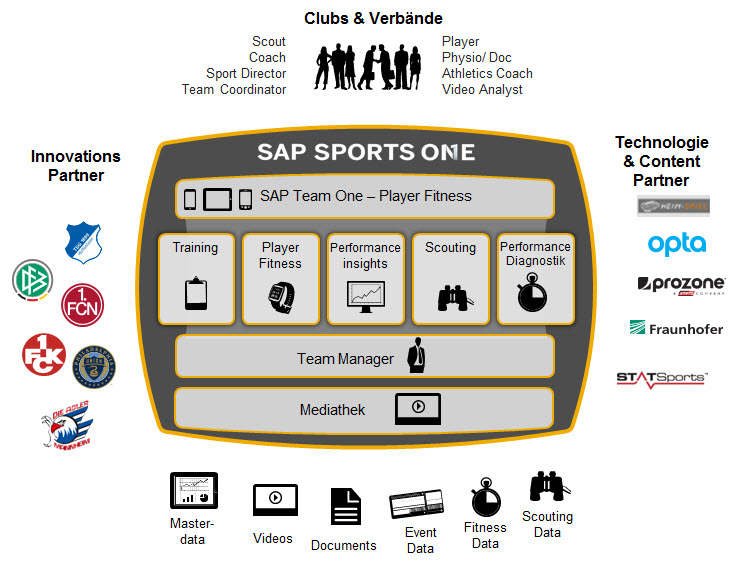
\includegraphics[scale=0.575]{se-wa-jpg/sportsone}
\caption{Überblick über Sports One}
\label{sportsone}
\end{figure}

Sports One ist eine von SAP, speziell für die Sportbranche entwickelte Software-Lösung und bietet derzeit Funktionen in den Bereichen Team Management, Spiel- und Trainingsanalysen, Spielerfitness, Leistungsdiagnostik und Scouting, welche im Gesamtkontext in \vref{sportsone} dargestellt sind. Das Modell der \textit{Expected Goals} würde, wie in \vref{goals} hingewiesen, innerhalb des Scoutingsbereich integriert werden, wodurch Offensivspieler in einem neuen Maßstab bewertet werden können. Für die Entwicklung dieses zusätzlichen Features für den Kunden entstehen unterschiedliche Kosten, die nachfolgend exemplarisch aufgezeigt werden. Die Entwicklung des grundlegenden mathematischen Modelles zur Berechnung der Wahrscheinlichkeit eines Torerfolges, ohne Integration in das bestehende Produkt, nahm in etwa 50 Werktage und eine Mitarbeiterkapazität in Anspruch. Bei einem fiktiven internen Tagessatz von \textsf{1.500\euro} ergeben sich dadurch \textit{Erstellungkosten des Grundmodelles} in Höhe von \textsf{75.000\euro}. Die Spieldaten werden dazu vom Datenprovider Opta Sports (vgl. \vref{opta}) über einen Lizenzvertrag jährlich eingekauft, wobei diese Verträge jedoch direkt zwischen Verein und Datenprovider geschlossen werden. Sports One stellt dazu die entsprechenden Schnittstellen für den Datenimport in das System bereit. Die für das Modell zugrundeliegenden Daten wurden von Opta Sports zu Forschungszwecken kostenfrei bereitgestellt, sodass letztlich keine Kosten für den Einkauf von den Daten aus Sicht des Unternehmens entstehen. Um das Modell letztlich im Scoutingbereich von Sports One nutzen zu können, fallen weitere Entwicklungskosten an. So müsste ein entsprechende Benutzerfläche mit angebundener Anwendungslogik erstellt, sowie die Schnittstelle für den Datenimport für das Modell bereitgestellt werden. Ein Team von drei Mitarbeitern würde bis zur Auslieferung des Features schätzungsweise drei Monate (ca. 70 Werktage) benötigen, wodurch zusätzliche \textit{Erstellungskosten der Anwendung} in Höhe von \textsf{315.000\euro} ergeben. Nach der Auslieferung dieses Features an den Kunden entstehen geschätzte jährliche \textit{Support- und Wartungskosten} von \textsf{100.000\euro}. Des Weiteren muss innerhalb der Beratung und des Verkaufs der Gesamtlösung das neue Feature propagiert werden, wodurch weitere jährliche \textit{Kosten der Beratung und des Verkaufs} in Höhe von \textsf{100.000\euro} anfallen. \vref{calc} fasst dazu alle anfallenden Kosten zusammen und gibt einen Ausblick auf die nächsten Jahre.

\begin{table}[H]
\centering
\caption{Exemplarische Kalkulation}
\label{calc}
\begin{tabular}{|l|r|r|r|r|}
\hline
\multicolumn{1}{|c|}{\textbf{Kosten}} & \multicolumn{1}{c|}{\textbf{Jahr 1}} & \multicolumn{1}{c|}{\textbf{Jahr 2}} & \multicolumn{1}{c|}{\textbf{Jahr 3}} & \multicolumn{1}{c|}{\textbf{Jahr 4}} \\ \hline
Erstellungskst. d. Grundmodelles      & 75.000\euro                              & 0\euro                                   & 0\euro                                   & ...                                  \\ \hline
Erstellungskst. d. Anwendung          & 315.000\euro                             & 0\euro                                   & 0\euro                                   & ...                                   \\ \hline
Support- und Wartungskosten           & 100.000\euro                             & 100.000\euro                             & 100.000\euro                             & ...                                  \\ \hline
Kosten der Beratung \& Verkauf        & 100.000\euro                             & 100.000\euro                             & 100.000\euro                             & ...                                  \\ \hline
Summe                                 & \underline{590.000\euro}                             & \underline{200.000\euro} & \underline{200.000\euro}                            & ...                                  \\ \hline
\end{tabular}
\end{table}

In Jahr 1 fallen durch die einmalige Entwicklung des Modelles und der Anwendung, sowie der Integration in das Gesamtprodukt hohe Kosten an, die durch die Investition geschuldet sind. In den darauf folgenden Jahren entstehen lediglich Kosten durch der Beratung und des Verkaufs sowie durch den Support und die Wartung des Modelles. Dieses Feature verlangt keine Vereins-spezifischen Konfigurationen, sodass beispielsweise bei einer Anzahl von 40 Kunden, die Kosten des Modelles ab Jahr 2 pro Kunde sich jährlich auf \textsf{5.000\euro} belaufen, die wiederum durch den Verkauf des Gesamtproduktes (als jährliche Lizenz) ausreichend gedeckt werden. 


\paragraph{Sichtweise des Vereins}
Mit Hilfe eines solcher integrierten Anwendung im Scoutingbereich ergeben sich aus der Sicht eines Fußballvereines einige wirtschaftlichen Konsequenzen. Neben den Linzenzkosten des Sport One Produktes müssen auch Spieldaten über einen Datenprovide, wie Opta Sports, zu eingekauft werden, wodurch sich zunächst Ausgaben ergeben. Durch die Nutzung des Features der \textit{Expected Goals} und der dadurch resultierenden objektiven Bewertung eines Spielers, können im Gegenzug einige Kosten eingespart werden. Beispielsweise wird für die Suche nach einem neuen Mittelstürmer einige Scouts beauftragt, die auf der einen Seite dafür bezahlt werden müssen, auf der anderen durch die Fahrtkosten auf die entsprechenden Spiele auch weitere Kosten verursachen. Durch die Vorselektion der Spieler anhand dieses neuen KPIs, wird die Auswahl der in Frage kommenden Spieler deutlich resultiert und somit folgich auch die Anzahl der benötigten Scouts, sodass Kosten eingespart werden. Letztlich muss ein Spieler jedoch immer vor einer Verpflichtung subjektiv eingeschätzt werden, da dieser auch beispielsweise von der Persönlichkeit in die Teamstruktur passen muss, was durch objektive Kennzahlen nicht gemessen werden kann. Des Weiteren können dadurch verborgene Talente entdeckt werden, die in einem frühen Stadium noch zu einem geringen Preis verpflichtet werden und einige Jahre später durch einen Verkauf an einen internationalen Top-Verein Millionen einbringen können, wodurch sich die Investition in diese Software-Lösung ausreichend gelohnt hätte. Wie in den genannten Beispielen aus dem Bereich des Baseballs und des Basketballs (vgl. \vref{goals}) ist es im Fußball nicht möglich eine Mannschaft, bestehend aus elf Spielern, anhand dieser einzelnen Kennzahl vollständig zusammen zu stellen, da in einem solchen Mannschaftssport weitere Faktoren, wie taktisches Verständnis oder Teamfähigkeit, eine wichtige Rolle einnehmen. 